\chapter{DESENVOLVIMENTO}

\section{Análise de circuitos}

Neste primeiro momento, será revisado o conceito de análise de circuitos. Para isso, devemos encontrar a resistência equivalente entre os pontos AB e CD do circuito \ref{fig:AnaliseDeCircuitos}

\begin{figure}[ht]
    \centering
    \fbox{
        \parbox{0.975\textwidth}{
            \centering
            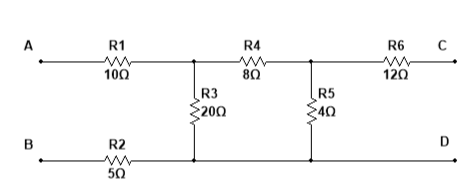
\includegraphics[width=0.975\textwidth]{images/analise_de_circuitos.png}
        }}
    \caption{Análise de circuitos}
    \vspace{-0.3cm}
    \label{fig:AnaliseDeCircuitos}
\end{figure}

\noindent
\textbf{Resolução}

\begin{Resolucao}[ht]
    \fbox{
        \parbox{0.975\textwidth}{
            \vspace{0.40cm}
            \centering
            Resistência equivalente AB:
            \[ ((8+4) // 20) + 10 + 5 = \textcolor{red}{22.5\Omega} \]

            Resistência equivalente CD:
            \[ (8+20) // 4 + 12 = \textcolor{red}{15.5\Omega} \]
        }
    }
    \captionof*{Resolucao}{Resolução: Circuito 01}
    \label{res:AnaliseDeCircuitos}
\end{Resolucao}

\section{Divisor de tensão}

Neste segundo momento, será revisado o conceito de divisor de tensão. Para isso, devemos encontrar a tensão de saída do circuito \ref{fig:DivisorDeTensao}

\begin{figure}[H]
    \centering
    \fbox{
        \parbox{0.975\textwidth}{
            \centering
            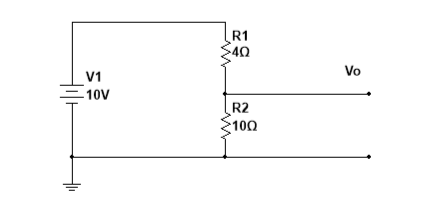
\includegraphics[width=0.975\textwidth]{images/divisor_de_tensao.png}
        }}
    \caption{Divisor de tensão}
    \vspace{-0.3cm}
    \label{fig:DivisorDeTensao}
\end{figure}

\noindent
\textbf{Resolução}

\begin{Resolucao}[H]
    \fbox{
        \parbox{0.975\textwidth}{
            \centering
            \[IT = \frac{V}{R1 + R2} \rightarrow \frac{10}{4 + 10} \simeq \textcolor{red}{714mA} \]
            Para se calcular a tensão sobre um resisstor, é necessário utilizar \\
            a divisão de Tensão $\rightarrow$ $\frac{R1}{R1+R2}$ * VT
            \[VR2 = \frac{10}{10 + 4} * 10V \rightarrow \simeq \textcolor{red}{7.14V} \]
            \[IVR2 = \frac{7.14}{10} = \textcolor{red}{714mA} \]
            (Mesmo resultado da Corrente Total, pois corrente em série é igual.)
        }
    }
    \captionof*{Resolucao}{Resolução: Circuito 02}
    \label{res:UmaMalha}
\end{Resolucao}

Através da imagem \ref{fig:DivisorDeTensao} podemos verificar os resultados obtidos por simulação

\begin{figure}[H]
    \centering
    \fbox{
        \parbox{0.975\textwidth}{
            \centering
            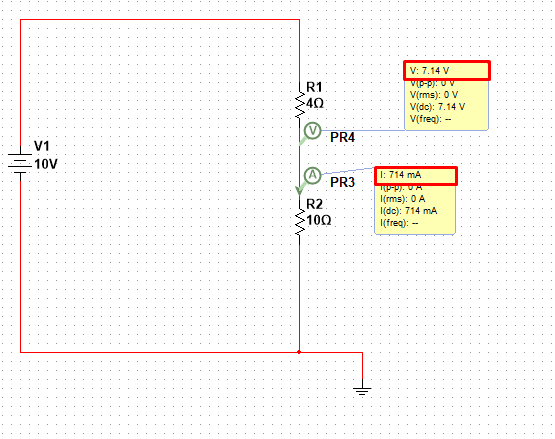
\includegraphics[width=0.975\textwidth]{images/simulacoes/divisor_de_tensao.png}
        }}
    \caption{Simulação do circuito de divisor de tensão}
    \vspace{-0.3cm}
    \label{fig:DivisorDeTensao}
\end{figure}

Com a tabela \ref{tab:ComparacaoDivisorDeTensao} podemos comparar os resultados obtidos por simulação com os resultados obtidos por cálculo, na qual comprovam que os cálculos estavam corretos.

\begin{quadro}[H]
    \centering
    \caption{Comparação entre os resultados obtidos por simulação e por cálculo do circuito de divisor de tensão}
    \begin{tabular}{|C{0.34\textwidth}|C{0.19\textwidth}|C{0.19\textwidth}|C{0.19\textwidth}|C{0.19\textwidth}|}
        \hline
        \rowcolor[HTML]{C0C0C0}
        \textbf{Modelo\textbackslash{}Variáveis} & \textbf{IT} & \textbf{VR2} & \textbf{IVR2} \\
        \hline
        Calculado & 714mA & 7.14V & 714mA \\
        \hline
        Simulado & 714mA & 7.14V & 714mA \\
        \hline
    \end{tabular}
    \vspace{-0.6cm}
    \label{tab:ComparacaoDivisorDeTensao}
\end{quadro}

\section{Divisor de corrente}

Neste terceiro momento, será revisado o conceito de divisor de corrente. Para isso, devemos encontrar a corrente de saída do circuito \ref{fig:DivisorDeCorrente}

\begin{figure}[H]
    \centering
    \fbox{
        \parbox{0.975\textwidth}{
            \centering
            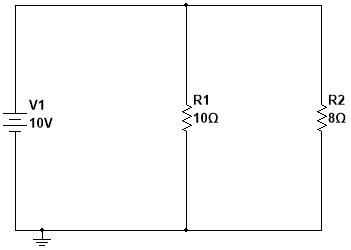
\includegraphics[width=0.975\textwidth]{images/divisor_de_corrente.png}
        }}
    \caption{Divisor de corrente}
    \vspace{-0.3cm}
    \label{fig:DivisorDeCorrente}
\end{figure}

\noindent
\textbf{Resolução}

\begin{Resolucao}[H]
    \fbox{
        \parbox{0.975\textwidth}{
            \centering
            \[IT = \frac{V}{R1 // R2}\rightarrow IT = \frac{10}{4.44} \simeq \textcolor{red}{2.25A}\]
            Para se calcular a divisão de corrente, utilizamos a seguinte fórmula: 
            \[I1 = \frac{R2}{R2 + R1} * IT \rightarrow \frac{8}{8 + 10} * 2.25A = \textcolor{red}{1.0A} \]
            \[I2 = \frac{R1}{R1 + R2} * IT \rightarrow \frac{10}{10 + 8} * 2.25A = \textcolor{red}{1.25A} \]
        }
    }
    \captionof*{Resolucao}{Resolução: Circuito 03}
    \label{res:UmaMalha}
\end{Resolucao}

Através da imagem \ref{fig:SimulacaoDivisorDeCorrente} podemos verificar os resultados obtidos por simulação

\begin{figure}[H]
    \centering
    \fbox{
        \parbox{0.975\textwidth}{
            \centering
            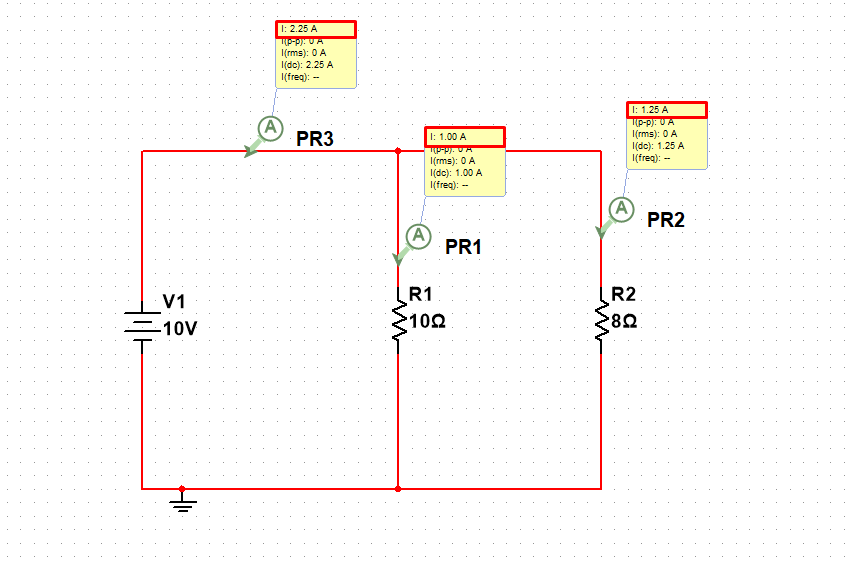
\includegraphics[width=0.975\textwidth]{images/simulacoes/divisor_de_corrente.png}
        }}
    \caption{Simulação do circuito de divisor de corrente}
    \vspace{-0.3cm}
    \label{fig:SimulacaoDivisorDeCorrente}
\end{figure}

Com a tabela \ref{tab:ComparacaoDivisorDeCorrente} podemos comparar os resultados obtidos por simulação com os resultados obtidos por cálculo, na qual comprovam que os cálculos estavam corretos.

\begin{quadro}[H]
    \centering
    \caption{Comparação entre os resultados obtidos por simulação e por cálculo do circuito de divisor de corrente}
    \begin{tabular}{|C{0.34\textwidth}|C{0.19\textwidth}|C{0.19\textwidth}|C{0.19\textwidth}|}
        \hline
        \rowcolor[HTML]{C0C0C0}
        \textbf{Modelo\textbackslash{}Variáveis} & \textbf{IT} & \textbf{I1} & \textbf{I2} \\
        \hline
        Calculado & 2.25A & 1.0A & 1.25A \\
        \hline
        Simulado & 2.25A & 1.0A & 1.25A \\
        \hline
    \end{tabular}
    \vspace{-0.6cm}
    \label{tab:ComparacaoDivisorDeCorrente}
\end{quadro}

\section{Malhas}

Neste seção de malhas, será abordado dois circuitos, sendo um deles com apenas uma malha, e outro com duas malhas no mesmo circuito.

\subsection{Uma Malha}

\begin{figure}[H]
    \centering
    \fbox{
        \parbox{0.975\textwidth}{
            \centering
            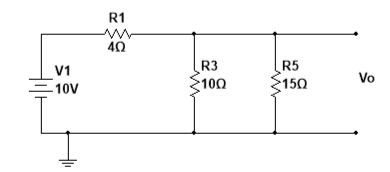
\includegraphics[width=0.975\textwidth]{images/malhas.png}
        }}
    \caption{Circuito com uma malha}
    \vspace{-0.3cm}
    \label{fig:UmaMalha}
\end{figure}

\noindent
\textbf{Resolução}

\begin{Resolucao}[H]
    \fbox{
        \parbox{0.975\textwidth}{
            \vspace{0.40cm}
            \centering
            Para calcular as correntes, é utilizado o divisor de corrente $\rightarrow$ $\frac{R2}{R1+R2}$ * IT \\
            \[I1 =  (\frac{15}{15 + 10}) * 1 \rightarrow \textcolor{red}{0.6A} \]
            \[I2 = (\frac{10}{10 + 15}) * 1 \rightarrow \textcolor{red}{0.4A} \]
            \[IT = I1 +I2 \rightarrow 0.6A + 0.4A = \textcolor{red}{1.0A} \]
            Para se calcular a tensão, é necessário utilizar a divisão de Tensão $\rightarrow$ $\frac{R1}{R1+R2}$ * VT \\
            \[Vo = \frac{15 // 10}{15 // 10 + 4} * 10 \rightarrow  \textcolor{red}{6V}\]
        }
    }
    \captionof*{Resolucao}{Resolução: Circuito 04}
    \label{res:UmaMalha}
\end{Resolucao}

Através da imagem \ref{fig:SimulacaoUmaMalha} podemos verificar os resultados obtidos por simulação

\begin{figure}[H]
    \centering
    \fbox{
        \parbox{0.975\textwidth}{
            \centering
            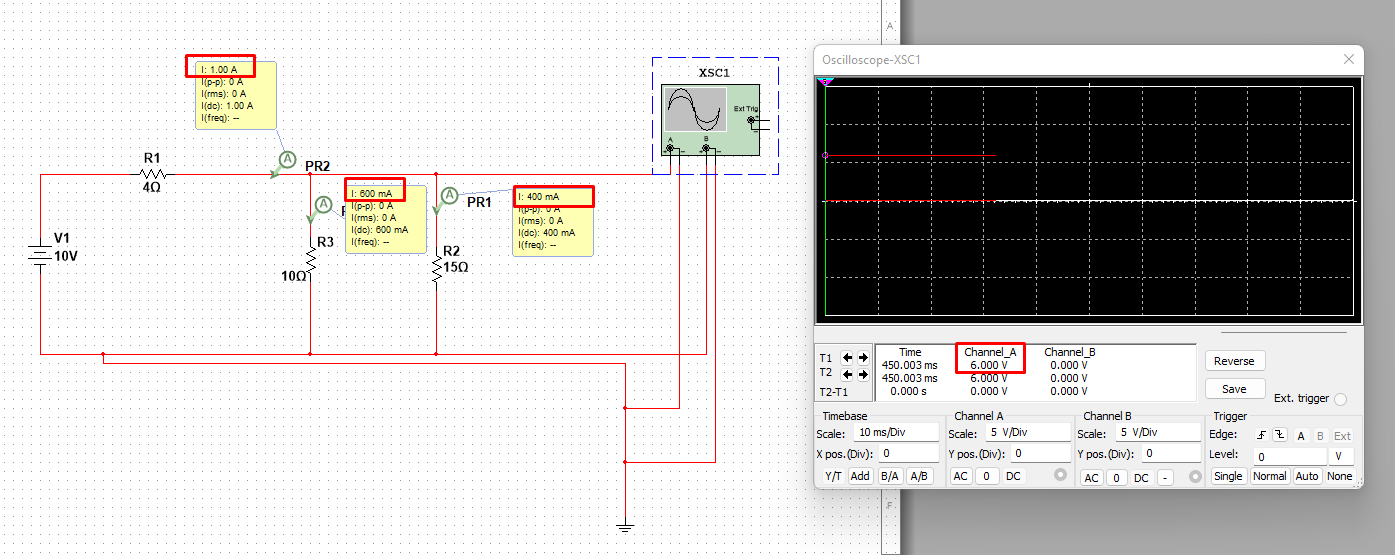
\includegraphics[width=0.975\textwidth]{images/simulacoes/1_malha.png}
        }}
    \caption{Simulação do circuito com uma malha}
    \vspace{-0.3cm}
    \label{fig:SimulacaoUmaMalha}
\end{figure}

Com a tabela \ref{tab:ComparacaoUmaMalha} podemos comparar os resultados obtidos por simulação com os resultados obtidos por cálculo, na qual comprovam que os cálculos estavam corretos.

\begin{quadro}[H]
    \centering
    \caption{Comparação entre os resultados obtidos por simulação e por cálculo do circuito com uma malha}
    \begin{tabular}{|C{0.35\textwidth}|C{0.14\textwidth}|C{0.14\textwidth}|C{0.14\textwidth}|C{0.14\textwidth}|}
        \hline
        \rowcolor[HTML]{C0C0C0}
        \textbf{Modelo\textbackslash{}Variáveis} & \textbf{I1} & \textbf{I2} & \textbf{IT} & \textbf{V0} \\
        \hline
        Calculado & 0.6A & 0.4A & 1.0A & 6V \\
        \hline
        Simulado & 0.6A & 0.4A & 1.0A & 6V \\
        \hline
    \end{tabular}
    \vspace{-0.6cm}
    \label{tab:ComparacaoUmaMalha}
\end{quadro}

\subsection{Duas Malhas}

Para realizar uma análise de um circuito com duas malhas, temos duas alternativas que serão abordadas a seguir:

\begin{enumerate}
    \item O método de malhas
    \item O método de superposição.
\end{enumerate}

\begin{figure}[H]
    \centering
    \fbox{
        \parbox{0.975\textwidth}{
            \centering
            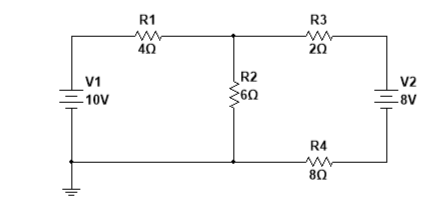
\includegraphics[width=0.975\textwidth]{images/2_malhas.png}
        }}
    \caption{Circuito com duas malhas}
    \vspace{-0.3cm}
    \label{fig:DuasMalhas}
\end{figure}

\noindent
\textbf{Resolução através do método de malhas}

\begin{Resolucao}[H]
    \fbox{
        \parbox{0.975\textwidth}{
            \centering
            \[M1 = V1 - 4I1 - 6(I1 + I2) = 0\] 
            \[M2 = V2 - 2I2 - 6(I2 + I1) - 8I2 = 0\] 

            \[M1 = 10I1 + 6I2 = 10 \rightarrow \textnormal{Multiplicamos por +6 para cortar I1}\]
            \[M2 = 6I1 + 16I2 = 8  \rightarrow \textnormal{Multiplicamos por -10 para cortar I1}\]
            
            \[M1 = \cancel{60I1} + 36I2 = 60\] 
            \[M2 = \cancel{-60I1} - 160I2 = -80\]

            \[M1 + M2 = -124I2 = 20 \]
            \[I2 = \frac{20}{124} \rightarrow \textcolor{red}{I2 = \frac{5}{31}A}\]

            \[\textnormal{Substituindo valor de I2 na M1\dots} \rightarrow 10I1 + 6(\frac{5}{31}) = 10 \]
            \[I1 \simeq \frac{9.03}{10} \rightarrow I1 \simeq \textcolor{red}{0.903A} \]

            \[\textnormal{Então \dots} IR2 = \frac{5}{31}A + 0.903A = \textcolor{red}{1.064A}\]
        }
    }
    \captionof*{Resolucao}{Resolução: Circuito 05 (Através do método de malhas)}
    \label{res:UmaMalha}
\end{Resolucao}

\noindent
\textbf{Resolução através do método de superposição}

\begin{Resolucao}[H]
    \fbox{
        \parbox{0.975\textwidth}{
            \centering
            Para o método de superposição, é necessário quebrar o circuito em duas partes, uma parte com V1 ligada e sem V2, e outra vez com V2 ligada e sem V1. \\
            Então, para o primeiro caso de apenas V1, temos: \\
            \[RE: (2 + 8 // 6) + 4 = 7.75\Omega \]
            \[IT: \frac{10}{7.75\Omega} \simeq 1.29 \]
            \[IR2: \frac{10}{10 + 6} * 1.29 \simeq \textcolor{red}{0.8A} \]

            Agora, considerando apenas a fonte V2 ligada, temos: \\
            \[RE = (4 // 6) + 2 + 8 = 12.4\Omega \]
            \[IT = \frac{8}{12.4} \simeq 0.645A \]
            \[IR2 = \frac{4}{10} * 0.645A \simeq \textcolor{red}{0.258A} \]    
            
            Por último, basta somar os valores de IR2 para obter o valor final: \\
            \[0.258A + 0.8A \simeq \textcolor{red}{1.058A}\]
        }
    }
    \captionof*{Resolucao}{Resolução: Circuito 05 (Através do método de superposição)}
    \label{res:UmaMalha}
\end{Resolucao}

Através da imagem \ref{fig:SimulacaoDuasMalha} podemos verificar os resultados obtidos por simulação

\begin{figure}[H]
    \centering
    \fbox{
        \parbox{0.975\textwidth}{
            \centering
            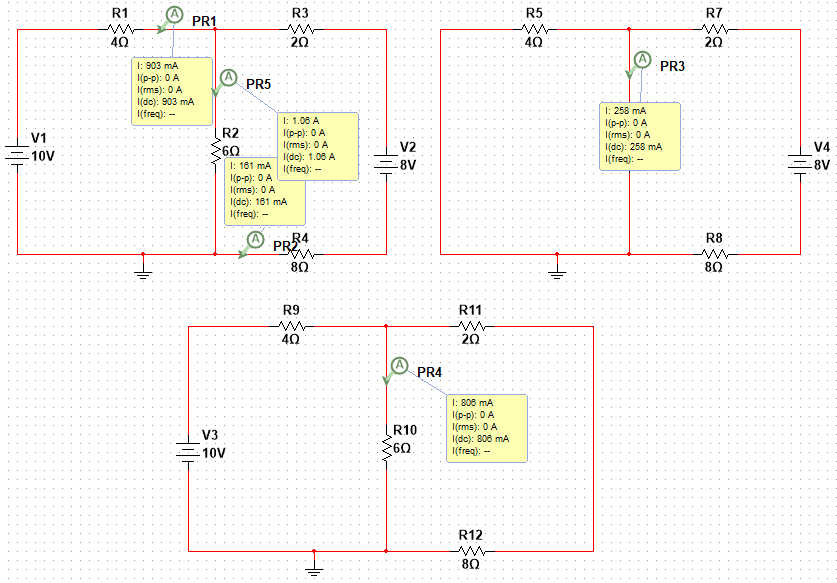
\includegraphics[width=0.975\textwidth]{images/simulacoes/2_malhas_separadas.png}
        }}
    \caption{Simulação do circuito com duas malhas}
    \vspace{-0.3cm}
    \label{fig:SimulacaoDuasMalha}
\end{figure}

Com a tabela \ref{tab:ComparacaoDuasMalha} podemos comparar os resultados obtidos por simulação com os resultados obtidos por cálculo, na qual comprovam que os cálculos estavam corretos, tendo apenas uma pequena diferença devido a aproximação dos valores.

\begin{quadro}[H]
    \centering
    \caption{Comparação entre os resultados obtidos por simulação e por cálculo do circuito com duas malhas}
    \begin{tabular}{|C{0.35\textwidth}|C{0.14\textwidth}|C{0.14\textwidth}|C{0.14\textwidth}|C{0.14\textwidth}|}
        \hline
        \rowcolor[HTML]{C0C0C0}
        \textbf{Modelo\textbackslash{}Variáveis} & \textbf{SP1.IR2} & \textbf{SP2.IR2} & \textbf{SPT.IR2} & \textbf{Malha.IR2} \\
        \hline
        Calculado & 0.800A & 0.258A & 1.058A & 1.064 \\
        \hline
        Simulado & 0.806A & 0.258A & 1.064A & 1.060 \\
        \hline
    \end{tabular}
    \vspace{-0.6cm}
    \label{tab:ComparacaoDuasMalha}
\end{quadro}